\documentclass[border=10pt]{standalone}
\usepackage{tikz}
\usetikzlibrary{shapes.geometric, arrows.meta, positioning, fit, backgrounds, calc}
\usepackage{mathptmx}

\definecolor{orchblue}{RGB}{70,130,180}
\definecolor{accgreen}{RGB}{76,153,0}
\definecolor{reducecolor}{RGB}{218,165,32}
\definecolor{lightgray}{RGB}{245,245,245}

\begin{document}
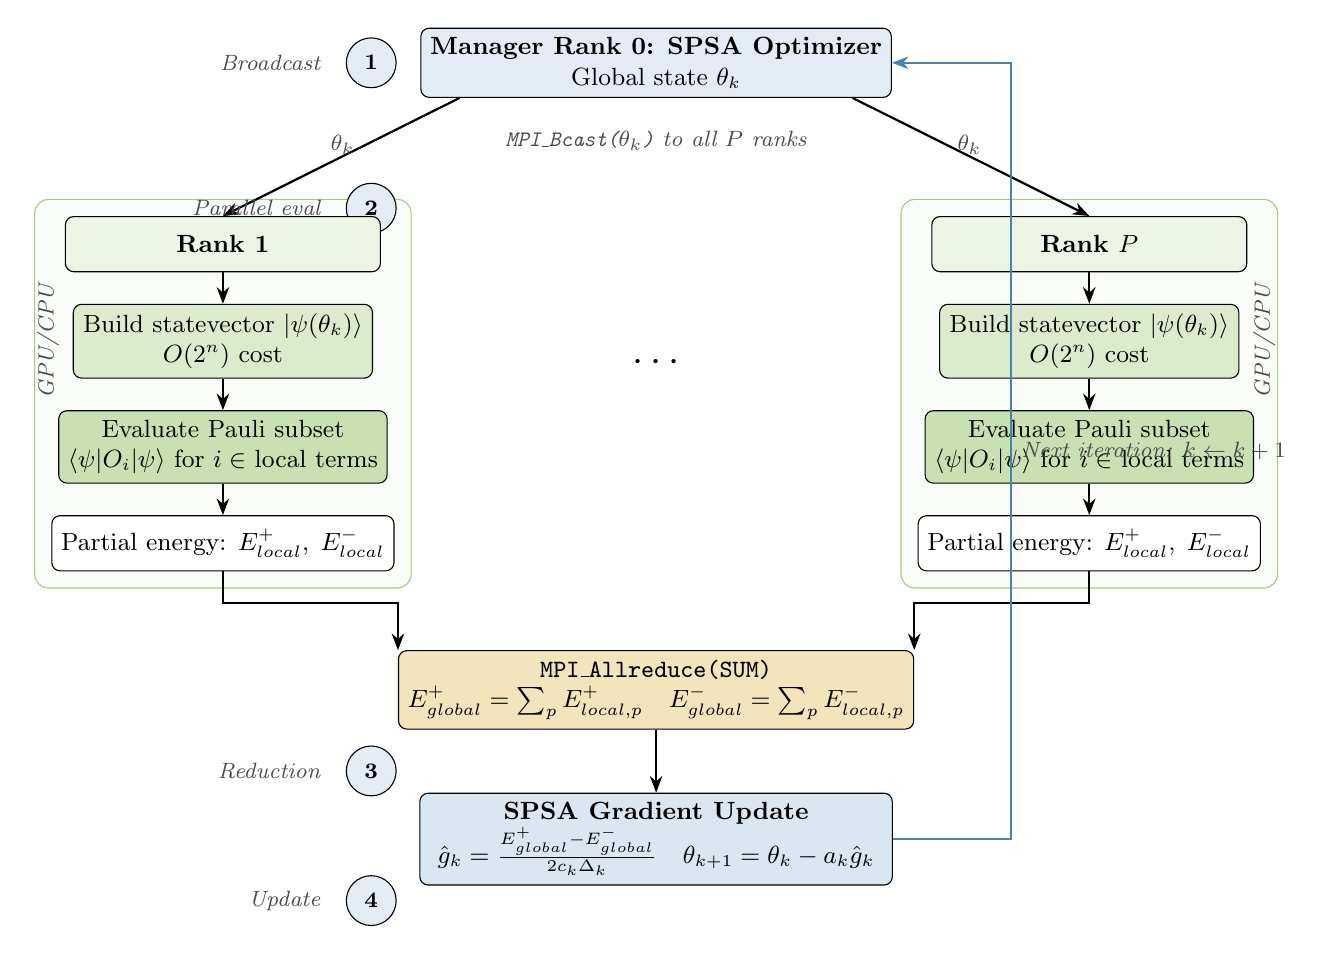
\begin{tikzpicture}[
    node distance=0.6cm and 2cm,
    every node/.style={font=\small},
    block/.style={rectangle, draw, rounded corners=3pt, minimum width=3.5cm, minimum height=0.7cm, align=center, fill=white},
    arrow/.style={-{Stealth[length=6pt]}, thick},
    label/.style={font=\footnotesize\itshape, text=gray!60!black},
    stepnum/.style={circle, draw, fill=orchblue!15, font=\footnotesize\bfseries, inner sep=2pt, minimum size=18pt},
]

% === STEP 1: Manager broadcasts ===
\node[stepnum] (s1) {1};
\node[block, fill=orchblue!15, right=0.3cm of s1, minimum width=5cm] (manager) {\textbf{Manager Rank 0: SPSA Optimizer}\\Global state $\theta_k$};

\node[label, below=0.3cm of manager] (bcast_label) {\texttt{MPI\_Bcast($\theta_k$)} to all $P$ ranks};

% === STEP 2: Workers compute locally ===
\node[stepnum, below=1.2cm of s1] (s2) {2};

\node[block, fill=accgreen!10, below left=1.5cm and 0.5cm of manager, minimum width=4cm] (rankA) {\textbf{Rank 1}};
\node[block, fill=accgreen!10, below right=1.5cm and 0.5cm of manager, minimum width=4cm] (rankB) {\textbf{Rank $P$}};

\draw[arrow] (manager.south west) ++(0.5,0) -- node[label, left, pos=0.4] {$\theta_k$} (rankA.north);
\draw[arrow] (manager.south east) ++(-0.5,0) -- node[label, right, pos=0.4] {$\theta_k$} (rankB.north);

% Rank A internals
\node[block, fill=accgreen!20, below=0.4cm of rankA, minimum width=3.8cm] (svA) {Build statevector $|\psi(\theta_k)\rangle$\\$O(2^n)$ cost};
\node[block, fill=accgreen!30, below=0.4cm of svA, minimum width=3.8cm] (pauliA) {Evaluate Pauli subset\\$\langle\psi|O_i|\psi\rangle$ for $i \in$ local terms};
\node[block, fill=white, below=0.4cm of pauliA, minimum width=3.8cm] (eA) {Partial energy: $E^+_{local},\; E^-_{local}$};

\draw[arrow] (rankA) -- (svA);
\draw[arrow] (svA) -- (pauliA);
\draw[arrow] (pauliA) -- (eA);

% Rank B internals
\node[block, fill=accgreen!20, below=0.4cm of rankB, minimum width=3.8cm] (svB) {Build statevector $|\psi(\theta_k)\rangle$\\$O(2^n)$ cost};
\node[block, fill=accgreen!30, below=0.4cm of svB, minimum width=3.8cm] (pauliB) {Evaluate Pauli subset\\$\langle\psi|O_i|\psi\rangle$ for $i \in$ local terms};
\node[block, fill=white, below=0.4cm of pauliB, minimum width=3.8cm] (eB) {Partial energy: $E^+_{local},\; E^-_{local}$};

\draw[arrow] (rankB) -- (svB);
\draw[arrow] (svB) -- (pauliB);
\draw[arrow] (pauliB) -- (eB);

% GPU labels
\node[label, left=0.05cm of svA] {\rotatebox{90}{GPU/CPU}};
\node[label, right=0.05cm of svB] {\rotatebox{90}{GPU/CPU}};

% Dots between
\node[draw=none] at ($(rankA.east)!0.5!(rankB.west)+(0,-1.5)$) {\Large$\cdots$};

% === STEP 3: Allreduce ===
\node[stepnum, below=6.5cm of s2] (s3) {3};
\node[block, fill=reducecolor!30, below=1cm of $(eA.south)!0.5!(eB.south)$, minimum width=6cm, minimum height=0.9cm] (reduce) {\textbf{\texttt{MPI\_Allreduce(SUM)}}\\$E^+_{global} = \sum_{p} E^+_{local,p}$\quad $E^-_{global} = \sum_{p} E^-_{local,p}$};

\draw[arrow] (eA.south) -- ++(0,-0.4) -| (reduce.north west);
\draw[arrow] (eB.south) -- ++(0,-0.4) -| (reduce.north east);

% === STEP 4: SPSA Update ===
\node[stepnum, below=1cm of s3] (s4) {4};
\node[block, fill=orchblue!20, below=0.8cm of reduce, minimum width=6cm] (update) {\textbf{SPSA Gradient Update}\\$\hat{g}_k = \frac{E^+_{global} - E^-_{global}}{2c_k\Delta_k}$\quad$\theta_{k+1} = \theta_k - a_k\hat{g}_k$};

\draw[arrow] (reduce) -- (update);

% Loop back
\draw[arrow, orchblue, thick] (update.east) -- ++(1.5,0) |- node[label, pos=0.25, right] {Next iteration: $k \leftarrow k+1$} (manager.east);

% Step labels on left
\node[label, left=0.2cm of s1] {Broadcast};
\node[label, left=0.2cm of s2] {Parallel eval};
\node[label, left=0.2cm of s3] {Reduction};
\node[label, left=0.2cm of s4] {Update};

% Background boxes for ranks
\begin{scope}[on background layer]
\node[rectangle, draw=accgreen!50, fill=accgreen!3, rounded corners=5pt, fit=(rankA)(svA)(pauliA)(eA), inner sep=6pt] {};
\node[rectangle, draw=accgreen!50, fill=accgreen!3, rounded corners=5pt, fit=(rankB)(svB)(pauliB)(eB), inner sep=6pt] {};
\end{scope}

\end{tikzpicture}
\end{document}
